\documentclass{article}
\usepackage{graphicx} % Required for inserting images
\usepackage[export]{adjustbox}% Required for inserting images
\usepackage{float}
\usepackage{placeins}
\title{PS04_myanswers_AG}
\author{Aryan Goyal}
\date{November 2023}

\begin{document}
\section{PS04 Answers}
Aryan Goyal

\noindent Student number: 18306046
\vspace{0.2cm}

\section{Question 1}
First, I run the following commands:
\begin{verbatim}
install.packages(car)
library(car)
data(Prestige)
help(Prestige)    
\end{verbatim}

\subsection{Answer 1a)}
I create a new variable "professional" by recoding the variable "type"
with professionals = 1 and white collar/blue collar workers = 0

\begin{verbatim}
Prestige$professional <- ifelse(Prestige$type == "prof", 1, 0)

# Inspecting the data and we can see our new variable
head(Prestige) 

\end{verbatim}

\subsection{Answer 1b)}
I run a multiple linear regression model with prestige as the outcome variable and three explanatory variables: income, professional and the interaction term of income x professional

\begin{verbatim}
    q1 <- lm(prestige~income+
                  professional+
                  income*professional, data=Prestige) 
summary(q1) 
\end{verbatim}

\begin{table}[h!] \centering 
  \caption{Multiple linear regression model} 
  \label{} 
\begin{tabular}{@{\extracolsep{5pt}}lc} 
\\[-1.8ex]\hline 
\hline \\[-1.8ex] 
 & \multicolumn{1}{c}{\textit{Dependent variable:}} \\ 
\cline{2-2} 
\\[-1.8ex] & prestige \\ 
\hline \\[-1.8ex] 
 income & 0.003$^{***}$ \\ 
  & (0.0005) \\ 
  & \\ 
 professional & 37.781$^{***}$ \\ 
  & (4.248) \\ 
  & \\ 
 income:professional & $-$0.002$^{***}$ \\ 
  & (0.001) \\ 
  & \\ 
 Constant & 21.142$^{***}$ \\ 
  & (2.804) \\ 
  & \\ 
\hline \\[-1.8ex] 
Observations & 98 \\ 
R$^{2}$ & 0.787 \\ 
Adjusted R$^{2}$ & 0.780 \\ 
Residual Std. Error & 8.012 (df = 94) \\ 
F Statistic & 115.878$^{***}$ (df = 3; 94) \\ 
\hline 
\hline \\[-1.8ex] 
\textit{Note:}  & \multicolumn{1}{r}{$^{*}$p$<$0.1; $^{**}$p$<$0.05; $^{***}$p$<$0.01} \\ 
\end{tabular} 
\end{table}


\begin{figure} %%Code to put figures in the pdf
    \centering
    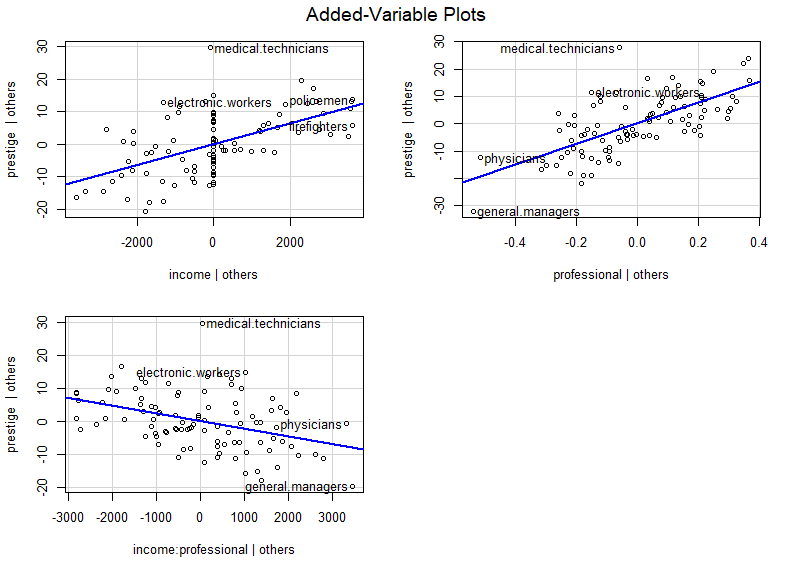
\includegraphics[width=1.25\textwidth]{Q1 Add Variable Plot.png}
    \caption{Add variable plots for Multiple linear Regression Model}
    \label{fig:enter-label}
\end{figure}
%%Replace the "%" with \ to use

\pagebreak
\subsection{Answer 1c)}
Based on 1b)
I come up with the following prediction equation:
\vspace{0.2cm}

\noindent $Prestige = 21.1422589 + (0.0031709*income) + (37.7812800*professional) - (0.0023257(income*professional))$

\subsection{Answer 1d)}

The coefficient for income is significant at the 0.001 level. Holding other explanatory variables constant, a 1 dollar increase in income
leads to a 0.0031709 scale points increase in Prestige on average. 

\subsection{Answer 1e)}

The coefficient for professional is significant at the 0.001 level.
Holding other explanatory variables constant, we can say that the
prestige score for professionals is 37.7812800 scale points higher than 
the prestige score for non-professionals on average

\subsection{Answer 1f)}
What is the effect of a \$1,000 increase in income on prestige score for professional occupations? when professional = 1.
Calculate the change in $\hat{y}$ associated with a \$1,000 increase in income based on your answer for (c)

\vspace{0.2cm}
Equation 1 where the income is \$1000:

\noindent $Prestige = 21.1422589 + (0.0031709*1000) + (37.7812800*1)  - (0.0023257(1000*1))$

$= 59.7687389$
    
Equation 2 where income increases by \$1000:

\noindent $Prestige = 21.1422589 + 0.0031709*2000 + 37.7812800*1 -0.0023257(2000*1)$

$= 60.6139389$    


\noindent Based on the 2 above equations, the difference between them represents the 
change in y-hat associated with a \$1000 increase in income:
\vspace{0.1cm}

\begin{math}
60.6139389 - 59.7687389 = 0.8452    
\end{math}
\\
Therefore, A \$1000 increase in income corresponds to a 0.8452 scale points increase in prestige based on our multiple linear regression model when the job is categorized as professional.

I do the same using R:
\begin{verbatim}
    coefficients <- coef(q1)

# Find the coefficient of income and the interaction term for professional occupations
coefficient_income <- coefficients["income"]
coefficient_interaction <- coefficients["income:professional"]

# Calculate the change in predicted prestige for a $1,000 increase in income
change_in_prestige <- ((coefficient_income + coefficient_interaction) * 1000)

# Print the change in predicted prestige
print(change_in_prestige)
# We get the same value: 0.8452

\end{verbatim}

\subsection{Answer 1g)}
I find the marginal effect of professional jobs when the variable income takes the value of \$6,000:
\\
Equation 1 (for non-professional):
\\
\noindent $Prestige = 21.1422589 + (0.0031709*6000) + (37.7812800*0) -(0.0023257(6000*0))$
\\
$= 40.1676589$
\\
This is the predicted Prestige based on our multiple linear regression model if an individual is a non-professional with an income of 6000\$
\\
Equation 2 (for professionals):
\\
$Prestige = 21.1422589 + (0.0031709*6000) + (37.7812800*1) -(0.0023257(6000*1))$
\\
$= 63.9947389$
\\
This is the predicted Prestige based on our multiple linear regression model if an individual is a professional with an income of 6000\$
\\
The difference between the two equations represents the change in $\hat{y}$:
\\
63.9947389 - 40.1676589 = 23.82708
\\
Therefore, for a person earning \$6000, prestige increases by 23.82708 scale points if the job is categorized as professional, rather than non-professional,
\\

I do the same using R:
\begin{verbatim}
    data1g <- data.frame(income = 6000, professional = c(0, 1))
    prestige1g <- predict(q1, newdata = data1g)
    change1g <- diff(prestige1g)
    print(change1g)
# We get this value: 23.82703 
\end{verbatim}

\pagebreak

\section{Question 2}

\subsection{Answer 2a)}
Q2a) Use the results from a linear regression to determine whether having these yard signs in a precinct affects vote share (e.g., conduct a hypothesis test with $\alpha$ = .05).
\\
\noindent In order to find the partial effect of a predictor variable on our outcome variable, I use the t-test for estimated coefficients.
\\
\noindent My null hypothesis is that there is no discerible linear relationship between having yard signs in a precinct and vote share (after controlling for the effects of other predictor variables), $H_0: \beta_j = 0$ 
\\
\noindent My alternative hypothesis is that there is discernible linear relationship between the predictor variable and outcome variable, $H_a: 
\beta_j \neq 0 $
\\
First, I calculate the test statistic using the values in the provided regression results.
\\
$t = \frac{\hat{\beta_j}}{se_\beta j}$
\\
Hence, $t = \frac{0.042}{0.016}$
\\
Therefore, $t = 2.625$
\\
Next, we determine the degrees of freedom,
$df = n - k - 1$,
where n is the number of observations
and k is the number of predictors (excluding the intercept)
\\
Therefore, $df = 30 - 2 - 1$ = 27
\\
Based on the degrees of freedom and our chosen significance level ($\alpha=0.05$), I find the critical t-value
\\
Based on the t-distribution table, I find the two-tailed critical value to 
be 2.05 at 27 degrees of freedom. 
\\
I used the table from this website: 
(https://faculty.washington.edu/heagerty/Books/Biostatistics/TABLES/t-Tables/)
\\
The absolute value of my test statistic, 2.625 is greater than the 
critical value, 2.05. Therefore, we can reject the null hypothesis and 
find support for the alternative that there is a discernible linear 
relationship between precincts with yard signs and vote share
\\
%%begin{figure} %%Code to put figures in the pdf
    %centering
    %includegraphics[width=1.3\textwidth]{%%This is where I put the .png file}
    %caption{Y and X1}
    %label{fig:enter-label}
%end{figure}
%%Replace the "%" with \ to use

\subsection{Answer 2b)}
Q2b)Use the results to determine whether being next to precincts with these yard signs affects vote share (e.g., conduct a hypothesis test with $\alpha$ = .05)

Similar Q2a) I conduct the t-test for estimated coefficients

\noindent My null hypothesis is that there is no discernible linear relationship between having yard signs in the adjacent precinct and vote share (after controlling for the effects of other predictor variables), $H_0: \beta_j = 0$ 

\noindent My alternative hypothesis is that there is discernible linear relationship between the predictor variable and outcome variable, $H_a: 
\beta_j \neq 0 $

Based on the provided regression results, I calculate the test statistic:
$t = \frac{\hat{\beta_j}}{se_\beta j}$

$t= \frac{0.042}{0.013}$
$t = 3.2308$

Next, we determine the degrees of freedom,
$df = n - k - 1$

df = 76 - 2 - 1
df = 73

Based on the degrees of freedom and our chosen significance level ($\alpha=0.05$), I find the critical t-value

Based on the t-distribution table, I find the two-tailed critical value to be 1.99 at 73 degrees of freedom.

The absolute value of my test statistic, 3.2308 is greater than the 
critical value, 1.99 at 73 degrees of freedom. Therefore, we can reject the null hypothesis and find support for the alternative that there is a discernible linear relationship between being next to precincts with yard signs and vote share. 


\subsection{Answer 2c)}
I interpret the coefficient for the constant term substantively.
The y-intercept represents the value of the outcome variable when all predictor variables are equal to zero. In this case, this means that our y-interecept estimates the vote share if there were 0 lawn signs put up in any precincts. This means that Ken Cuccinelli's vote share would be 0.302 scale points if no lawn signs were put up.

On the basis of this, I calculate the percentage change in the outcome variable associated with the treatment condition compared to the baseline condition (represented by the constant term).
\\
$\frac{\beta_1} {\beta_0} * 100$ 
= $\frac{0.042}{0.302} * 100$
= $13.91\%$
\\
This value suggests that, on average, precincts where yard signs were put up had a 13.91\% higher vote share for Cuccinelli compared to the baseline where no yard signs were put up.

\subsection{Answer 2d)}
I evaluate the model fit for this regression using R-squared.
A $R^2$ value of 0.094 is low and suggests that the explanatory variables in the model do not explain much of the variance in the outcome variable. This $R^2$ value indicates that only 9.4\% of the variance in the outcome variable is explained by the explanatory variables in our multiple linear regression model.  
This is an indication that we should include other variables in our model that could explain the variation in vote share to a greater extent, other than whether precincts had yard signs.

\end{document}
